\section{实验}
\label{sec:experiments}

\subsection{数据集与评测协议}
\label{sec:datasets}

\paragraph{少标注跨域协议}
GWFSS 竞赛发布的少标注协议包含来自 9 个源域的 99 张像素级标注训练图像、64,368 张无标注训练图像和 99 张验证图像，另有来自未见域的 110 张测试图像；所有图像均被裁剪为 $512\times512$ 像素。该协议同时考查无标注数据利用和未知采集域泛化。模型选择、超参数调整和消融实验仅依据源域验证集完成，测试集仅用于最终评测，以避免目标域信息泄漏。除非另有说明，所有对比方法均使用相同的 99 张标注图像。

\paragraph{完整数据区域协议}
数据集论文给出的地域划分进一步检验了模型对特定少标注拆分的依赖程度。完整数据包含 1,096 张精细标注图像和 52,078 张无标注图像，覆盖 11 个研究机构、不同成像平台和约 $0.09$--$0.71$ mm/pixel 的地面采样距离 \citep{wang2025gwfss}。训练域来自 Arvalis、CIMMYT、ETHZ、INRAE、NJAU、RRES 和 ULiege，UTokyo 作为验证域，UQ 作为测试域。实验保持官方地域划分不变，并分别使用训练域中 10\%、25\%、50\% 和 100\% 的标注图像；各比例由固定随机种子分层采样，且在所有方法之间共享。不同采集条件下的局部标注细节见\cref{fig:dataset}，基于全部标注图像的域级统计与器官尺度负担分别见\cref{fig:domain-fingerprint,fig:organ-scale-burden}。

\begin{figure}[!htbp]
\centering
%\includegraphics[width=\linewidth]{figures/dataset_domains.pdf}
\fbox{\parbox{0.94\linewidth}{\centering \vspace{1.05cm}
\placeholder{数据域图版由四列三行构成，四列分别对应近距离高分辨率、远距离低分辨率、强阴影绿色冠层和衰老黄色冠层。第一行给出原始 RGB，第二行叠加背景、麦穗、茎秆和叶片的固定颜色标注，第三行显示相同位置的局部放大。列标题标记机构或域编号，底部短标签列出地面采样距离、生育阶段、视角和主要干扰。两个放大框分别定位叶茎交叠处的类别歧义，以及低分辨率下仅有 1--3 像素宽的茎秆。训练域采用实线边框，未知测试域采用虚线边框，图例注明该域在训练中不可见。}
\vspace{1.05cm}}}
\caption{GWFSS 不同采集域的图像、像素级标注与局部细节。实线框和虚线框分别表示源域与未知测试域，局部放大区域呈现了叶茎交叠和低分辨率细茎两类主要困难。}
\label{fig:dataset}
\end{figure}

\begin{figure*}[!htbp]
\centering
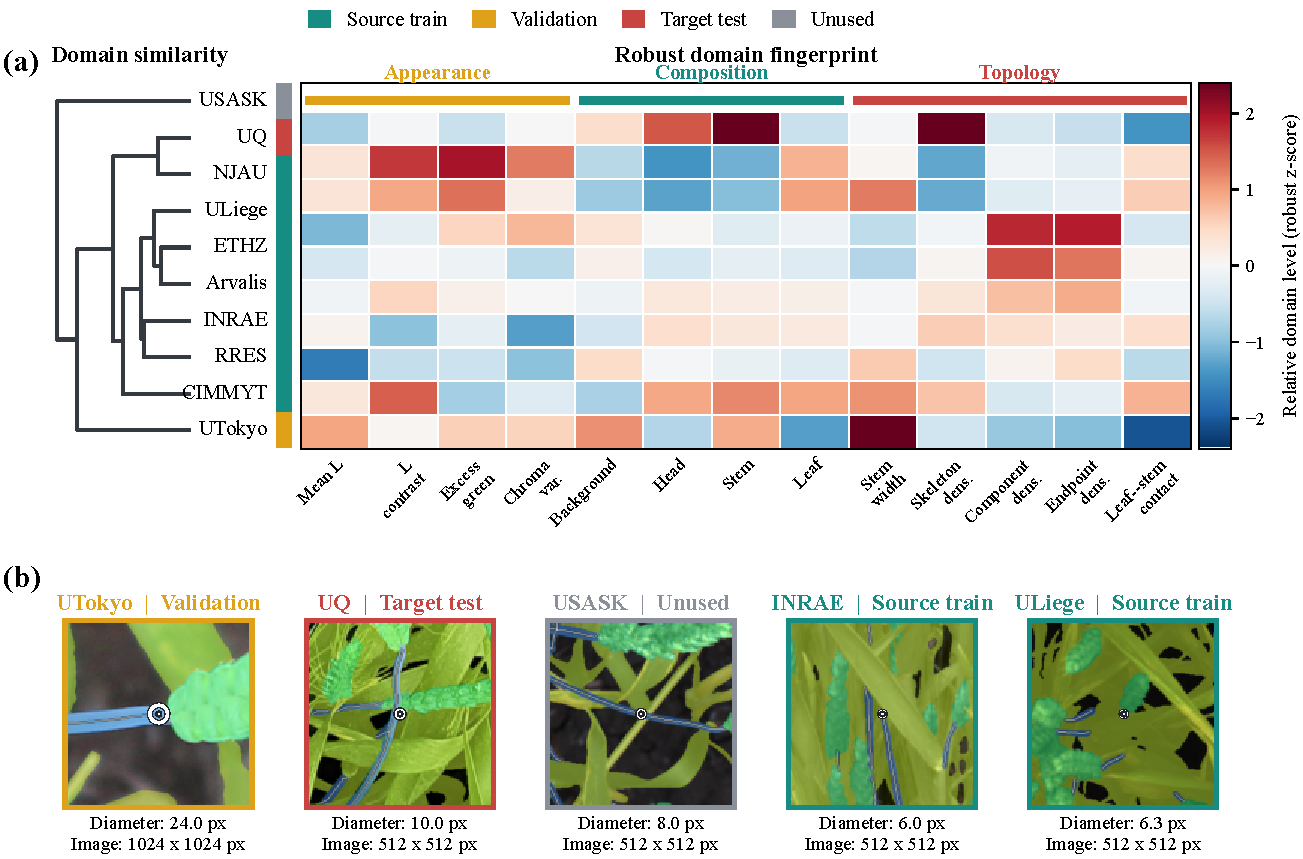
\includegraphics[width=\textwidth]{figures/domain_morphology_fingerprint.pdf}
\caption{完整标注子集的跨域外观、器官组成与拓扑形态指纹。(a) 对每个域的 13 项图像与标注统计取中位数，并以跨域中位数和四分位距标准化；树状图采用标准化指纹的欧氏距离和平均连接法。侧边色带表示该域在地域协议中的作用。(b) 在具有有效茎秆骨架的图像中，自动选取最接近各域中位指纹的样本，并以相同的 $256\times256$ 原生像素视野显示局部区域。白线表示茎秆中轴，圆环表示中位宽度测量点处的最大内切圆。绿色、蓝色和黄绿色叠加区域分别为麦穗、茎秆和叶片标注。}
\label{fig:domain-fingerprint}
\end{figure*}

用于上述统计的 1,096 张图像在标注子集中对应 10 个具有类别掩码的采集域。由\cref{fig:domain-fingerprint}可见，验证域 UTokyo 和目标测试域 UQ 到七个源域中心的标准化距离分别为 6.32 和 3.97，均超过任一单独源域到该中心的最大距离 3.27。UQ 的主要偏移同时出现在绿色过量指数（$+1.95$）、色度变化（$+1.58$）、亮度对比度（$+1.55$）和麦穗面积占比（$-1.41$）上，括号内为相对源域中心的稳健标准化差值。

图中的茎宽描述标注栅格上的局部直径，而非小麦茎秆的物理直径。对二值茎秆掩码进行骨架化后，以 $D(p)$ 表示骨架像素 $p$ 到最近背景像素的欧氏距离，单幅图像的茎宽定义为 $\operatorname{median}_{p\in S}2D(p)$，域级数值再取域内图像的中位数。UTokyo 标注图像为 $1024\times1024$，其余九个标注域为 $512\times512$；因此 UTokyo 的域中位宽度 22.8 px 与 UQ 代表样本的 10.0 px 不能直接解释为前者具有更粗的物理茎秆。该统计反映的是模型所需处理的原生栅格尺度变化，\cref{fig:domain-fingerprint}(b) 也据此采用固定原生像素大小的裁块，而不再把不同分辨率的整幅图像缩放到相同显示尺寸。结合器官面积占比和叶--茎接触统计可知，地域迁移同时改变了成像外观、器官组成和细长结构的像素表达，单纯的颜色增强无法覆盖后两类变化；本文因而在伪标签可靠性和跨域原型构建中显式保留器官拓扑信息。

\begin{figure*}[!htbp]
\centering
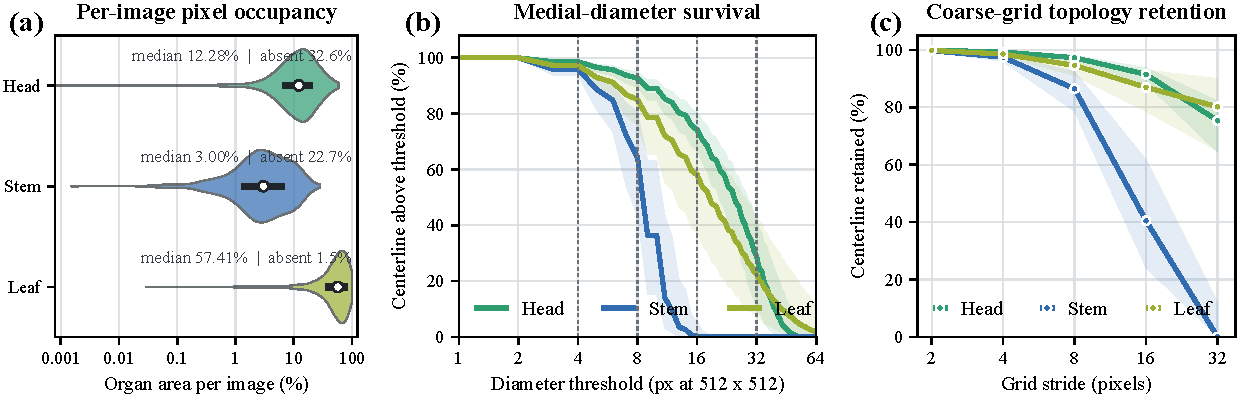
\includegraphics[width=\textwidth]{figures/organ_scale_burden.pdf}
\caption{统一尺度下的器官像素负担与几何生存性。(a) 每幅图像中非零器官面积占比的对数分布，白点和黑线分别表示中位数与四分位区间，文字同时给出器官缺失图像的比例。(b) 骨架局部直径生存曲线，即局部直径不小于给定阈值的中心线比例；实线和阴影分别为跨图像中位数与四分位区间，虚线标出常见特征步长。(c) 以网格内器官占比不低于 50\% 为保留条件，将真值投影到不同步长的粗网格后，原始中心线仍被覆盖的比例。所有掩码均以最近邻插值统一为 $512\times512$；粗网格投影仅用于几何诊断，不代表网络预测。}
\label{fig:organ-scale-burden}
\end{figure*}

器官占比和结构宽度呈现出一致的茎秆劣势，相关分布汇总于\cref{fig:organ-scale-burden}(a)。在器官实际出现的图像中，茎秆面积中位数仅为 3.00\%，麦穗和叶片则分别为 12.28\% 和 57.41\%。麦穗在 32.6\% 的图像中缺失，反映了数据覆盖多个生育期；即使排除器官缺失造成的零值，茎秆的像素监督仍明显少于另外两类器官。

将全部掩码统一到 $512\times512$ 后，茎秆、叶片和麦穗的图像级中位局部直径依次为 8.25、18.11 和 24.17 px。茎秆中心线中有 35.7\% 的局部直径不足 8 px，而叶片和麦穗的对应比例仅为 15.0\% 和 7.3\%。这种尺度差异在粗网格诊断中产生非线性后果：stride 8 时三类器官的中位中心线保留率分别为 86.4\%、94.6\% 和 97.2\%，stride 16 时茎秆骤降至 40.5\%，叶片和麦穗仍保持 87.0\% 和 91.5\%。多数栅格化没有模拟卷积特征的学习能力，但它排除了纹理和类别置信度的影响，单独揭示了离散采样对细长结构施加的几何压力。这一结果解释了为何茎秆监督需要保留稳定中心线，也说明局部放大应优先分配给发生结构断裂的区域，而不是均匀增加所有器官的推理分辨率。

\subsection{评价指标}

遵循数据集论文，本文以四类平均交并比（mIoU）作为主要指标，并同时报告背景、麦穗、茎秆和叶片的类别 IoU。类别 $c$ 的 IoU 定义为
\begin{equation}
\operatorname{IoU}_c=
\frac{\operatorname{TP}_c}
{\operatorname{TP}_c+\operatorname{FP}_c+\operatorname{FN}_c},
\qquad
\operatorname{mIoU}=\frac{1}{C}\sum_{c=1}^{C}\operatorname{IoU}_c .
\end{equation}
整体 mIoU 容易掩盖像素占比较低类别的变化，因此实验将茎秆 IoU 作为核心辅助指标。二值茎秆掩码上的 soft-clDice \citep{shit2021cldice}、骨架精确率、骨架召回率和边界 F-score 则分别度量中心线重合、结构检出和轮廓质量。所有结构指标采用相同的骨架化参数和边界容差。

效率评测报告参数量、FLOPs、单张图像延迟、峰值显存和分割器前向次数。延迟包含裁剪、窗口选择和局部结果融合，并在相同硬件、批大小及预热设置下测量。密集多尺度滑窗方法的前向次数按实际裁剪数统计，\BAZR 的对应计算量为 $1+K$ 次前向。

\subsection{实现细节}
\label{sec:implementation}

基础网络由 BEiTv2-Large、ViT-Adapter、Mask2Former 和 SAPA 构成 \citep{peng2022beitv2,chen2023vitadapter,cheng2022mask2former,lu2022sapa}。编码器采用 ImageNet-1K 预训练权重，输入裁剪尺寸为 $512\times512$。AdamW 优化器的解码器初始学习率为 $1\times10^{-4}$，编码器学习率乘子为 0.1，权重衰减为 0.05。监督预热和半监督联合训练分别执行 20,000 和 90,000 次迭代；联合训练的全局批大小为 2 张有标注图像和 2 张无标注图像。弱增强包括多尺度短边缩放、$512\times512$ 随机裁剪、SSD 颜色扰动和随机水平翻转，学生分支额外采用颜色抖动、随机灰度和高斯模糊。EMA 动量设为 0.9996，前 20,000 次联合训练迭代作为教师冻结阶段。

\TRPL 使用原尺度与 0.75 倍尺度两个教师视图，背景、麦穗、茎秆和叶片的置信阈值依次为 0.70、0.70、0.55 和 0.70。不确定性权重 $\beta$ 和温度 $\tau_u$ 分别为 1.0 和 0.5，最大可接受不确定性为 0.75；骨架阈值、持续性阈值和边界半径分别为 0.35、0.5 和 2 像素。区域 Dice、拓扑和骨架一致性损失的权重依次为 0.5、0.5 和 0.25。\TCPM 使用 9 组域记忆，原型动量 $\mu$ 为 0.99，对比温度 $\tau_p$ 为 0.1，每类每次最多采样 256 个核心像素，留出域每 1,000 次迭代轮换一次。对比、域紧致和困难负样本损失的权重分别为 0.1、0.05 和 0.05。\BAZR 从步长为 128 的 $256\times256$ 候选窗口中选择 $K=4$ 个区域，将其放大到 $512\times512$，NMS 阈值设为 0.3；熵、异常端点、尺度分歧和茎秆概率的路由权重依次为 1.0、2.0、1.0 和 0.5。

所有主结果采用 3 个固定随机种子报告均值与标准差。训练和推理在 NVIDIA A100 上完成，代码基于 PyTorch 1.9.0、CUDA 11.1 和 Detectron2 0.6 实现。

\subsection{与现有方法的比较}

\paragraph{少标注跨域结果}
Cao 等人的方法结合 Guided Distillation、器官分布筛选和密集多尺度滑窗，在验证集与未知域测试集上分别取得 77.04\% 和 74.68\% mIoU \citep{cao2025detailminority}。DeCon 通过持续预训练、无标注样本选择和不确定性过滤得到 73.61\% 和 67.88\% \citep{ghosh2025decon}。统一主干监督基线、两种已有方法和本文方法的结果汇总于\cref{tab:small-label-main}，其中结构指标与实际前向次数用于区分训练收益和测试时计算收益。

\begin{table*}[!htbp]
\centering
\caption{GWFSS 少标注跨域协议上的定量比较。mIoU、Stem IoU 和 clDice 的单位为百分数，``--'' 表示原论文未报告相应结果，前向次数按每张 $512\times512$ 测试图像统计。}
\label{tab:small-label-main}
\resizebox{\textwidth}{!}{
\begin{tabular}{lccccccc}
\toprule
方法 & 主干网络 & 使用无标注数据 & 验证 mIoU & 测试 mIoU & Stem IoU & Stem clDice & 前向次数 \\
\midrule
监督基线 & BEiTv2-L & 否 & \placeholder{XX.XX} & \placeholder{XX.XX} & \placeholder{XX.XX} & \placeholder{XX.XX} & 1 \\
DeCon \citep{ghosh2025decon} & ConvNeXt-L/BEiT-L & 是 & 73.61 & 67.88 & -- & -- & -- \\
Cao 等 \citep{cao2025detailminority} & BEiTv2-L & 是 & 77.04 & 74.68 & -- & -- & $\sim160$ \\
\METHOD（全局推理） & BEiTv2-L & 是 & \placeholder{XX.XX} & \placeholder{XX.XX} & \placeholder{XX.XX} & \placeholder{XX.XX} & 1 \\
\METHOD（\BAZR） & BEiTv2-L & 是 & \placeholder{XX.XX} & \placeholder{XX.XX} & \placeholder{XX.XX} & \placeholder{XX.XX} & 5 \\
\bottomrule
\end{tabular}}
\end{table*}

监督基线从验证域迁移到未知测试域时下降了 \placeholder{X.XX} 个百分点，而 \METHOD 将该差距缩小到 \placeholder{X.XX} 个百分点，并相对监督基线提高测试 mIoU \placeholder{X.XX} 个百分点。这一变化表明性能增益并非只来自对 99 张标注图像的进一步拟合。对细长结构的改善更为集中：Stem IoU、clDice 和边界 F-score 分别提高 \placeholder{X.XX}、\placeholder{X.XX} 和 \placeholder{X.XX} 个百分点。clDice 的增幅高于边界 F-score，说明主要收益来自茎秆断裂的减少，而非预测区域的均匀膨胀。

全局推理与 \BAZR 共享完全相同的模型权重，两者的测试 mIoU 相差 \placeholder{X.XX} 个百分点，因而该增益可以归因于局部高分辨率细化。默认 $K=4$ 时每幅图像仅执行 5 次分割器前向，相比密集多尺度滑窗约 160 次前向减少了 96.9\% 的调用；实测延迟由 \placeholder{XXXX ms} 降至 \placeholder{XXX ms}。精度和计算量的共同变化说明，结构风险能够比均匀滑窗更有效地分配测试时预算。

\paragraph{完整数据区域泛化结果}
地域划分比随机拆分更直接地暴露采集域偏移。数据集论文中，SegFormer-B1 的 mIoU 为 60.64\%，其中茎秆 IoU 仅为 19.23\%；DeepLabV3+ 的两项结果分别为 52.15\% 和 6.64\% \citep{wang2025gwfss}。同一划分上的统一主干监督基线与 \METHOD 结果也列入\cref{tab:region-main}，从而控制网络容量差异。

\begin{table}[!htbp]
\centering
\caption{完整 GWFSS 数据地域划分上的类别 IoU 与 mIoU（\%）。}
\label{tab:region-main}
\resizebox{\linewidth}{!}{
\begin{tabular}{lccccc}
\toprule
方法 & 背景 & 麦穗 & 茎秆 & 叶片 & mIoU \\
\midrule
DeepLabV3+ \citep{wang2025gwfss} & 74.32 & 46.25 & 6.64 & 81.40 & 52.15 \\
SegFormer-B1 \citep{wang2025gwfss} & 75.46 & 66.11 & 19.23 & 81.75 & 60.64 \\
统一主干监督基线 & \placeholder{XX.XX} & \placeholder{XX.XX} & \placeholder{XX.XX} & \placeholder{XX.XX} & \placeholder{XX.XX} \\
\METHOD & \placeholder{XX.XX} & \placeholder{XX.XX} & \placeholder{XX.XX} & \placeholder{XX.XX} & \placeholder{XX.XX} \\
\bottomrule
\end{tabular}}
\end{table}

在未知地域上，\METHOD 相对统一主干监督基线提高 mIoU \placeholder{X.XX} 个百分点，其中茎秆获得最大的类别增益 \placeholder{X.XX} 个百分点；背景和叶片分别变化 \placeholder{X.XX} 和 \placeholder{X.XX} 个百分点。类别间的不均匀增益与 \TCPM 的采样机制一致。大面积器官从收缩后的内部区域已能得到稳定原型，而像素稀少的茎秆从中心线核心中获益更明显，边界混合像素对其类别中心的牵引随之减弱。源域平均 mIoU 仅变化 \placeholder{X.XX} 个百分点，最差源域和未知域则分别提高 \placeholder{X.XX} 和 \placeholder{X.XX} 个百分点。这组差异进一步表明，原型约束主要改善了跨域稳定性，而非对易分源域提供一般性的容量增益。

\subsection{消融实验}
\label{sec:ablation}

\paragraph{三个模块的增量作用}
模块消融从同一监督基线出发，并保持主干、数据和训练预算不变。训练阶段依次引入 \TRPL 与 \TCPM，\BAZR 只改变推理路径，因此启用 \TCPM 的最后两组共享模型权重。各模块带来的增量结果见\cref{tab:module-ablation}。

\begin{table*}[!htbp]
\centering
\caption{三个模块在少标注协议上的增量消融。$\checkmark$ 表示启用对应模块，所有指标均在相同数据划分下计算。}
\label{tab:module-ablation}
\begin{tabular}{ccccccccc}
\toprule
\TRPL & \TCPM & \BAZR & 验证 mIoU & 测试 mIoU & Stem IoU & Stem clDice & Boundary F & 前向次数 \\
\midrule
 & & & \placeholder{XX.XX} & \placeholder{XX.XX} & \placeholder{XX.XX} & \placeholder{XX.XX} & \placeholder{XX.XX} & 1 \\
$\checkmark$ & & & \placeholder{XX.XX} & \placeholder{XX.XX} & \placeholder{XX.XX} & \placeholder{XX.XX} & \placeholder{XX.XX} & 1 \\
$\checkmark$ & $\checkmark$ & & \placeholder{XX.XX} & \placeholder{XX.XX} & \placeholder{XX.XX} & \placeholder{XX.XX} & \placeholder{XX.XX} & 1 \\
$\checkmark$ & $\checkmark$ & $\checkmark$ & \placeholder{XX.XX} & \placeholder{XX.XX} & \placeholder{XX.XX} & \placeholder{XX.XX} & \placeholder{XX.XX} & 5 \\
\bottomrule
\end{tabular}
\end{table*}

引入 \TRPL 后，Stem IoU 和 clDice 分别提高 \placeholder{X.XX} 和 \placeholder{X.XX} 个百分点，而 mIoU 增幅为 \placeholder{X.XX} 个百分点。结构指标更显著的变化表明，区域平均指标确实弱化了细茎连续性的改善。进一步加入 \TCPM 后，源域验证与未知域测试 mIoU 分别变化 \placeholder{X.XX} 和 \placeholder{X.XX} 个百分点；更大的测试域增益符合域级记忆对未知条件的约束作用。在相同权重上启用 \BAZR 又将 Stem IoU 提高 \placeholder{X.XX} 个百分点。逐图错误分析显示，\TRPL 消除的训练噪声断裂与 \BAZR 修复的推理断裂仅有 \placeholder{XX.X\%} 重合，说明二者处理的是互补误差，而非重复优化同一批样本。

\paragraph{伪标签结构设计}
固定阈值、多视图不确定性和中心线--区域解耦使用相同的教师预测，差别仅在伪标签进入损失的方式。源域验证标签在训练期间保持隐藏，只用于离线计算接纳率和中心线准确率。具体结果汇总于\cref{tab:trpl-ablation}。

\begin{table}[!htbp]
\centering
\caption{伪标签可靠性建模的消融结果。接纳率衡量进入无监督损失的像素比例，中心线准确率在隐藏的验证标注上离线计算。}
\label{tab:trpl-ablation}
\resizebox{\linewidth}{!}{
\begin{tabular}{lcccc}
\toprule
伪标签策略 & 接纳率 & 中心线准确率 & Stem IoU & clDice \\
\midrule
固定类别阈值 & \placeholder{XX.XX} & \placeholder{XX.XX} & \placeholder{XX.XX} & \placeholder{XX.XX} \\
熵不确定性 & \placeholder{XX.XX} & \placeholder{XX.XX} & \placeholder{XX.XX} & \placeholder{XX.XX} \\
多视图不确定性 & \placeholder{XX.XX} & \placeholder{XX.XX} & \placeholder{XX.XX} & \placeholder{XX.XX} \\
中心线--区域解耦（\TRPL） & \placeholder{XX.XX} & \placeholder{XX.XX} & \placeholder{XX.XX} & \placeholder{XX.XX} \\
\bottomrule
\end{tabular}}
\end{table}

单纯采用熵过滤使接纳率由 \placeholder{XX.XX\%} 变为 \placeholder{XX.XX\%}，但中心线准确率只提高 \placeholder{X.XX} 个百分点，表明像素置信度无法充分区分边界模糊与位置错误。多视图分歧进一步排除了跨尺度不稳定区域，中心线准确率提高到 \placeholder{XX.XX\%}。完整 \TRPL 在保持 \placeholder{XX.XX\%} 接纳率的同时，将 Stem IoU 和 clDice 分别提高 \placeholder{X.XX} 和 \placeholder{X.XX} 个百分点，断裂组件数下降 \placeholder{XX.X\%}。接纳率并未与结构指标同步增加，说明收益来自监督证据的重新组织，而非简单扩大伪标签覆盖范围。

\paragraph{原型来源与域泛化}
原型消融逐步改变均值计算所使用的像素集合，并单独移除留一域模拟。除平均性能外，实验还记录最差源域 mIoU，以降低样本量和域难度差异对平均值的掩盖。不同原型证据的比较见\cref{tab:prototype-ablation}。

\begin{table}[!htbp]
\centering
\caption{原型证据来源与留一域训练的消融结果。最差源域 mIoU 为各源域独立评测结果中的最小值。}
\label{tab:prototype-ablation}
\resizebox{\linewidth}{!}{
\begin{tabular}{lccc}
\toprule
原型策略 & 验证 mIoU & 最差源域 mIoU & 测试 mIoU \\
\midrule
无原型 & \placeholder{XX.XX} & \placeholder{XX.XX} & \placeholder{XX.XX} \\
完整高置信区域 & \placeholder{XX.XX} & \placeholder{XX.XX} & \placeholder{XX.XX} \\
收缩内部区域 & \placeholder{XX.XX} & \placeholder{XX.XX} & \placeholder{XX.XX} \\
拓扑核心，无留一域模拟 & \placeholder{XX.XX} & \placeholder{XX.XX} & \placeholder{XX.XX} \\
拓扑核心与留一域模拟（\TCPM） & \placeholder{XX.XX} & \placeholder{XX.XX} & \placeholder{XX.XX} \\
\bottomrule
\end{tabular}}
\end{table}

完整高置信区域原型的测试 mIoU 为 \placeholder{XX.XX\%}，去除边界像素后提高到 \placeholder{XX.XX\%}，证实混合边界会偏移类别中心。用器官特异的拓扑核心替代统一收缩区域后，最差源域和未知域 mIoU 又分别提高 \placeholder{X.XX} 和 \placeholder{X.XX} 个百分点；与此同时，茎秆域级原型到全局原型的平均距离由 \placeholder{X.XXX} 降至 \placeholder{X.XXX}，茎秆与叶片原型间距增加 \placeholder{X.XXX}。表示距离与分割性能的同向变化支持了“纯净结构核心收紧跨域类别分布”的解释。移除留一域模拟仅使源域均值变化 \placeholder{X.XX} 个百分点，却使未知域结果下降 \placeholder{X.XX} 个百分点，说明轮换留出主要作用于域外泛化，而不是常规源域拟合。

\paragraph{精细化策略的精度--效率权衡}
所有精细化策略复用同一模型权重，性能变化仅来自计算位置和预算。实验以单尺度和密集滑窗作为两个计算端点，并比较仅熵路由与完整断裂感知路由。端点覆盖率表示被选窗口覆盖异常骨架端点的比例，路由结果及其延迟列于\cref{tab:routing-ablation}。

\begin{table}[!htbp]
\centering
\caption{局部精细化策略的精度--效率比较。端点覆盖率和分割指标以百分数表示，延迟包含窗口评分、裁剪和融合。}
\label{tab:routing-ablation}
\resizebox{\linewidth}{!}{
\begin{tabular}{lccccc}
\toprule
推理策略 & $K$ & mIoU & Stem IoU & 端点覆盖率 & 延迟（ms） \\
\midrule
全局单尺度 & 0 & \placeholder{XX.XX} & \placeholder{XX.XX} & -- & \placeholder{XXX} \\
仅熵路由 & 4 & \placeholder{XX.XX} & \placeholder{XX.XX} & \placeholder{XX.XX} & \placeholder{XXX} \\
\BAZR & 2 & \placeholder{XX.XX} & \placeholder{XX.XX} & \placeholder{XX.XX} & \placeholder{XXX} \\
\BAZR & 4 & \placeholder{XX.XX} & \placeholder{XX.XX} & \placeholder{XX.XX} & \placeholder{XXX} \\
\BAZR & 8 & \placeholder{XX.XX} & \placeholder{XX.XX} & \placeholder{XX.XX} & \placeholder{XXX} \\
密集多尺度滑窗 \citep{cao2025detailminority} & $\sim159$ & \placeholder{XX.XX} & \placeholder{XX.XX} & 100.00 & \placeholder{XXXX} \\
\bottomrule
\end{tabular}}
\end{table}

仅熵路由覆盖了 \placeholder{XX.XX\%} 的异常端点，但其中 \placeholder{XX.XX\%} 的窗口落在叶片或麦穗的普通高熵边界。引入端点密度和内部尺度差异后，端点覆盖率达到 \placeholder{XX.XX\%}，Stem IoU 随之提高 \placeholder{X.XX} 个百分点。这一结果表明分类不确定性与结构失效并不等价，显式结构信号减少了对普通器官边界的无效放大。随着 $K$ 从 2 增至 8，mIoU 增益由 \placeholder{X.XX} 增至 \placeholder{X.XX} 个百分点，而延迟近似线性增长；$K=4$ 之后的边际收益仅为 \placeholder{X.XX} 个百分点。剩余误差因而更多来自类别混淆和全局上下文缺失，继续提高局部放大预算难以修复。默认配置以密集滑窗 \placeholder{XX.X\%} 的延迟取得相差 \placeholder{X.XX} 个百分点的 mIoU，体现了精度与计算成本之间的有效折中。

\subsection{定性分析与讨论}

\begin{figure*}[!htbp]
\centering
%\includegraphics[width=0.96\linewidth]{figures/qualitative_comparison.pdf}
\fbox{\parbox{0.94\linewidth}{\centering \vspace{1.15cm}
\placeholder{定性比较图采用六行七列布局，列依次为 RGB、真值、监督基线、现有半监督基线、加入 TRPL、加入 TCPM 和完整 TopoWheat。六行覆盖 1--3 像素宽细茎、叶茎交叠、叶片遮挡造成的真实可见中断、衰老黄色器官、杂草与残体背景以及未知域低分辨率图像。所有预测以固定类别颜色和相同透明度叠加于 RGB，每行使用相同位置的局部放大框。红色箭头标记漏分断裂，黄色箭头标记叶茎混淆，白色箭头标记错误跨遮挡连接，完整方法中的绿色轮廓标记被恢复的可见茎秆。最后一行保留完整方法仍然失败的案例，各子图下方给出对应的 Stem IoU 和 clDice。}
\vspace{1.15cm}}}
\caption{不同模块在典型困难场景中的定性比较。箭头分别标识茎秆断裂、叶茎混淆和跨遮挡误连，最后一行呈现完整方法的代表性失败案例。}
\label{fig:qualitative}
\end{figure*}

\begin{figure*}[!htbp]
\centering
%\includegraphics[width=0.96\linewidth]{figures/diagnostic_analysis.pdf}
\fbox{\parbox{0.94\linewidth}{\centering \vspace{1.05cm}
\placeholder{机制诊断图横向分为 A、B、C 三个面板。面板 A 对同一无标注样本给出固定阈值伪标签、多视图不确定性、稳定中心线、忽略边界和离线真值；局部放大区域标记固定阈值删除的真实茎秆与 TRPL 排除的错误茎秆，底部列出接纳率和中心线准确率。面板 B 使用相同 UMAP 参数并排呈现无原型与拓扑核心原型的嵌入，点形状区分背景、麦穗、茎秆和叶片，颜色深浅区分采集域，大号标记表示域级与全局原型；右下角小图比较类内跨域距离和茎秆--叶片间距。面板 C 依次给出熵热图、端点热图、内部尺度差异、综合路由分数、Top-$K$ 窗口和融合结果，并并排呈现仅熵路由误选的叶片边界与完整路由命中的中等熵断茎。三个面板共享样本编号、类别颜色和箭头图例。}
\vspace{1.05cm}}}
\caption{可靠伪标签、跨域原型和结构风险路由的机制诊断。三个面板分别对应监督证据筛选、特征空间聚合和局部计算分配。}
\label{fig:diagnostic}
\end{figure*}

典型困难场景中的局部预测汇总于\cref{fig:qualitative}。监督基线主要出现低分辨率细茎断裂和叶茎交叠处的类别替换。拓扑可靠伪标签学习减少了固定阈值造成的细茎漏分，同时没有跨越真实遮挡补全不可见部分。在衰老器官与未知域图像中，原型记忆明显抑制了叶茎互换，说明改善并非局限于边界平滑。选择性放大的修正集中在全局预测已经出现异常端点的区域，原本正确的叶片和麦穗边界大多保持不变。

这些视觉现象由\cref{fig:diagnostic}中的中间量进一步解释。多视图稳定中心线避开了宽度不确定的茎秆边界，拓扑核心原型缩小了同类特征的域间距离，并扩大茎秆与叶片的类别间距；综合路由分数则命中了熵值不高但端点异常的断茎。可视化与接纳率、原型距离和端点覆盖率的量化变化一致，从不同层面连接了三个模块的作用机制。

按地面采样距离、生育阶段和茎秆像素占比进行的分组统计显示，\TRPL 在低茎秆占比组中提高 clDice \placeholder{X.XX} 个百分点，\TCPM 在域偏移最大的分组中提高 mIoU \placeholder{X.XX} 个百分点，\BAZR 收益与异常端点密度呈正相关（$r=\placeholder{X.XX}$，$p=\placeholder{X.XXX}$）。逐图配对检验和 95\% 置信区间排除了少量视觉样例主导平均结果的可能，困难分组中的集中增益也与各模块的设计目标一致。

误差分析同时揭示了方法的边界。当多个茎秆在低分辨率下完全重合时，多视图预测可能保持一致却仍然错误，稳定中心线无法恢复输入中已经消失的实例信息。固定 $K$ 假设图像具有近似的细化需求，因而在简单图像上产生少量冗余计算，并在结构极复杂的图像中遗漏部分困难区域。遮挡场景中的另一类错误来自拓扑监督对前景关系的误判；虽然本文只分割可见器官且不显式连接两个可见端点，完整方法仍产生 \placeholder{XX} 个跨叶片误连，较监督基线减少 \placeholder{XX.X\%}。这些失败表明，图像自适应预算和显式遮挡关系建模仍是进一步提高结构分割可靠性的关键方向。
